\clearpage
\section*{\hfil ВВЕДЕНИЕ \hfil}
	В современной добыче полезных ископаемых активно применяются средства математического моделирования для симуляции процессов, происходящих в пласте. Однако на данный момент полноценное моделирование не представляется возможным, поэтому используются различные приближенные методы. Для правильной симуляции процессов, происходящих в недрах, необходимо смоделировать саму среду, в которой эти процессы протекают. Обычно, данные о структуре среды доступны только в некотором количестве точек (скважин), в которых непосредственно идет добыча. Есть мотивация для попыток использования методов машинного обучения для синтеза моделей среды, похожих на существующие в природе. Так как геологические среды часто имеют пространственно скоррелированные неоднородности, то в рамках решения проблемы синтеза геологоподобной среды возникает задача синтезирования текстур с трендами.
	
	Под текстурой с трендом в данном случае понимается изображение, в котором есть изменение некоторой статистической характеристики вдоль одного из направлений. Такими характеристиками, например, могут быть изменение интенсивности появления частиц среды или пористости среды.
	
	Базовым подходом в задаче синтеза текстур на данный момент является использование искусственных нейросетей. Однако, известные работы в области синтеза текстур с помощью искусственных нейросетей \cite{texture-synthesis-using-CNN, texture-networks} показывают, что у нейросетевых моделей есть проблемы с воспроизведением формы объектов, а также различных пространственно скоррелированных структур. Соответственно, целью данной работы ставится поиск нейросетевой архитектуры, способной улавливать и воспроизводить протяженные корреляции.
	
	Для упрощения задачи, будем в дальнейшем рассматривать множество изображений с трендами, удовлетворяющее следующим ограничениям:
	
	\begin{itemize}
		\item Монохромные изображения 256 x 256 пикселей
		\item Изменяющимся свойством является интенсивность появления частиц $\lambda$
		\item Тренд является линейным и направлен вдоль оси изображения $z_1$: 
		$ \lambda = \lambda_{init} + k z_1 $
		\item По оси $z_2$ остается равномерное распределение частиц
	\end{itemize}
	
	Каждый такой тренд фиксируется значениями $\lambda_{init}$ и $\lambda_{final}$. Следовательно, 
	$$k = \frac{\lambda_{final} - \lambda_{init}}{256}$$
	Пример такого изображения с трендом интенсивности приведен на (Рис. \ref{1-trend-example}):
	
	\begin{figure}[h]
		\centering{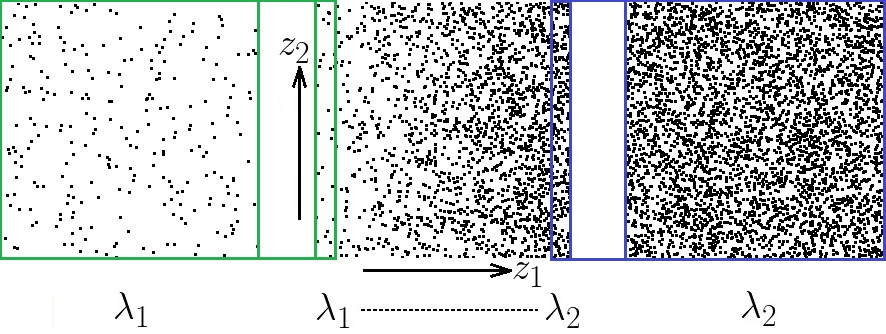
\includegraphics[width=\linewidth]{1-introduction/trend-example}}
		\caption{Пример изображения с трендом, фиксируемого двумя изображениями}
		\label{1-trend-example}
	\end{figure}
	
	Математически сформулировать постановку описанной задачи можно с помощью так называемой вероятностной постановки задачи обучения \cite{Voron-ML, GAN-original}.
	
	Рассмотрим многомерное пространство $X$, содержащее множество всех изображений $x$: $X = \{x\}$. Пусть у нас есть обучающая выборка из изображений, содержащих в себе рассматриваемое множество трендов $D = \{x_i\}$. Тогда считается, что  обучающая выборка изображений с трендами $D$ задает в этом пространстве вероятностное распределение $P_X : X \longrightarrow [0,1]$, устроенное таким образом, что точки, соответствующие изображениям из выборки, имеют высокую вероятность, а остальные - низкую. Таким образом, с математической точки зрения задача синтеза текстуры с трендом сводится к синтезу случайного изображения $x'$, принадлежащего распределению, близкому к задаваемому обучающей выборкой:
	$$ P_{X'} \approx P_X, \quad x' \sim X'$$
	
	``Классический'' статистический подход к решению подобного рода задач заключается в введении в рассмотрение параметризированного семейства распределений вероятности и его подстройке к имеющимся данным:
	
	\begin{itemize}
		\item Вводится параметризированное семейство распределений вероятности $P_{\theta}(x)$
		\item Параметры $\theta$ находятся из обучающей выборки:
		$$ \mathcal{L}_{\theta}(D) = \prod_{x \in D} P_{\theta}(x) $$
		$$ \theta^{*} = \underset{\theta}{\arg\max} \mathcal{L}_{\theta}(D)$$
		\item Генерируется объект (изображение) из распределения $ P_{\theta^{*}}$
	\end{itemize}
	
	Этот подход приводит к проблемам:
	
	\begin{itemize}
		\item Пространство параметров $\theta$ может быть огромной размерности
		\item Известной параметрической модели распределения может не существовать
	\end{itemize}
	
	Простой пример объекта со сложным пространством параметров - человеческое лицо. Задачу генерации изображения реалистичного человеческого лица долгое время не могли решить с удовлетворительным качеством. Однако последние достижения в области искусственных нейронных сетей привели к существенному улучшению качества генеративных моделей самого разнообразного типа. В частности, впечатляющие результаты были достигнуты с помощью генеративных состязательных сетей (GAN) \cite{cGAN, cGAN-face, EBGAN, BEGAN}, что мотивирует попытку применения нейросетей этой архитектуры в поставленной задаче.
	
	\subsection*{Постановка задачи}
	
	Таким образом, для достижения обозначенной во введении цели, поставить задачу работы можно так:
	
	\begin{itemize}
		\item Разработать модифицированные для синтеза описанного множества текстур с трендами архитектуры нейронных сетей
		\item Провести вычислительные эксперименты, связанные с обучением нейросетей (то есть, с решением задач многопараметрической оптимизации)
		\item Синтезировать с помощью обученных нейросетей новые текстуры и верифицировать их
	\end{itemize}